\begin{tabular}{M{6.5cm}M{11cm}}
	\textbf{LỚP CÔ THẢO - THẦY SANG}& \textbf{ĐỀ ÔN TẬP KIỂM TRA CUỐI HỌC KÌ 1}\\
	\textbf{MÃ ĐỀ: 005}& \textbf{Bài thi môn: VẬT LÝ 12}\\
	\textit{(Đề thi có 05 trang)}& \textit{Thời gian làm bài: 50 phút, không kể thời gian phát đề}
	
	\noindent\rule{4cm}{0.8pt} \\
\end{tabular}
\setcounter{section}{0}
\section{Câu trắc nghiệm nhiều phương án lựa chọn}
\textit{Thí sinh trả lời từ câu 1 đến câu 18. Mỗi câu hỏi thí sinh chọn một phương án}
\setcounter{ex}{0}
\Opensolutionfile{ans}[ans/G12-5-TN]
% ===================================================================
\begin{ex}
Đặc điểm nào sau đây là của sự bay hơi?	
	\choice
	{Chỉ xảy ra đối với một số ít chất lỏng}
	{Xảy ra với tốc độ như nhau ở mọi nhiệt độ}
	{\True Xảy ra ở bất kì nhiệt độ nào của chất lỏng}
	{Chỉ xảy ra trong lòng chất lỏng}
	\loigiai{}
\end{ex}
% ===================================================================
\begin{ex}
	Tính chất nào sau đây \textbf{không phải} của phân tử vật chất ở thể khí
	\choice
	{Chuyển động không ngừng}
	{\True Chuyển động hỗn loạn xung quanh các vị trí cân bằng cố định}
	{Nhiệt độ càng cao các phân tử chuyển động càng nhanh}
	{Chuyển động hỗn loạn}
	\loigiai{}
\end{ex}
% ===================================================================
\begin{ex}
Nhiệt độ không tuyệt đối $\left(\SI{0}{\kelvin}\right)$ là nhiệt độ mà tại đó các phân tử có	
	\choice
	{động năng chuyển động nhiệt bằng không và thế năng tương tác giữa chúng là cực đại}
	{động năng chuyển động nhiệt cực đại và thế năng tương tác giữa chúng là cực đại}
	{\True động năng chuyển động nhiệt bằng không và thế năng tương tác giữa chúng là tối thiểu}
	{động năng chuyển động nhiệt cực đại và thế năng tương tác giữa chúng là bằng không}
	\loigiai{}
\end{ex}
% ===================================================================
\begin{ex}
	Nếu hai vật có nhiệt độ khác nhau được đặt tiếp xúc nhau thì
	\choice
	{quá trình truyền nhiệt dừng lại khi nhiệt độ một vật đạt $\SI{0}{\celsius}$}
	{quá trình truyền nhiệt dừng lại khi nhiệt năng hai vật bằng nhau}
	{\True quá trình truyền nhiệt dừng lại khi nhiệt độ hai vật bằng nhau}
	{quá trình truyền nhiệt dừng lại khi độ biến thiên nhiệt độ hai vật bằng nhau}
	\loigiai{}
\end{ex}
% ===================================================================
\begin{ex}
Trạng thái của một lượng khí lí tưởng xác định được xác định bởi	
	\choice
	{áp suất, thể tích và khối lượng}
	{\True áp suất, nhiệt độ và thể tích}
	{khối lượng mol, áp suất và nhiệt độ}
	{thể tích, nhiệt độ và số mol}
	\loigiai{}
\end{ex}
% ===================================================================
\begin{ex}
	Nhiệt độ cơ thể người là $\SI{37}{\celsius}$ sẽ tương ứng với nhiệt độ bao nhiêu trong thang đo nhiệt độ Kelvin?
	\choice
	{\True $\SI{310}{\kelvin}$}
	{$\SI{300}{\kelvin}$}
	{$\SI{236}{\kelvin}$}
	{$\SI{210}{\kelvin}$}
	\loigiai{}
\end{ex}
% ===================================================================
\begin{ex}
	Khi các nguyên tử, phân tử cấu tạo nên vật chuyển động nhanh lên thì đại lượng nào sau đây tăng lên?
	\choice
	{Thế năng của vật tăng lên}
	{Khối lượng của vật}
	{Động năng của vật tăng lên}
	{\True Nhiệt độ của vật}
	\loigiai{}
\end{ex}
% ===================================================================
\begin{ex}
	Trong quá trình hít vào, cơ hoành và cơ liên sườn của một người co lại, mở rộng khoang ngực và hạ thấp áp suất không khí bên trong xuống dưới môi trường xung quanh để không khí đi vào qua miệng và mũi đến phổi. Giả sử phổi của một người chứa $\SI{6000}{\milli\liter}$ không khí ở áp suất $\SI{1}{atm}$. Nếu người đó mở rộng khoang ngực thêm $\SI{500}{\milli\liter}$ bằng cách giữ mũi và miệng đóng lại để không hít không khí vào phổi thì áp suất không khí trong phổi theo đơn vị $\si{atm}$ sẽ là bao nhiêu? Giả sử nhiệt độ không khí không đổi.
	\choice
	{\True $\SI{0.92}{atm}$}
	{$\SI{1.08}{atm}$}
	{$\SI{1.20}{atm}$}
	{$\SI{0.85}{atm}$}
	\loigiai{
	$$p_1V_1=p_2V_2\Leftrightarrow 1\cdot 6000=p_2\cdot 6500\Rightarrow p_2\approx\SI{0.92}{atm}.$$
	}
\end{ex}
% ===================================================================
\begin{ex}
	Một vật được làm bằng kim loại A có khối lượng $\SI{0.1}{\kilogram}$ ở nhiệt độ $\SI{100}{\celsius}$ được bỏ vào một nhiệt lượng kế làm bằng đồng có khối lượng $\SI{0.1}{\kilogram}$ chứa $\SI{0.2}{\kilogram}$ nước có nhiệt độ là $\SI{20}{\celsius}$. Khi cân bằng, nhiệt độ của hệ là $\SI{24}{\celsius}$. Biết nhiệt dung riêng của đồng là $\SI{380}{\joule/\kilogram\cdot\kelvin}$, của nước là $\SI{4200}{\joule/\kilogram\cdot\kelvin}$. Nhiệt dung riêng của kim loại A là
	\choice
	{$\SI{880}{\joule/\kilogram\cdot\kelvin}$}
	{$\SI{570}{\joule/\kilogram\cdot\kelvin}$}
	{$\SI{2062}{\joule/\kilogram\cdot\kelvin}$}
	{\True $\SI{462}{\joule/\kilogram\cdot\kelvin}$}
	\loigiai{
	Áp dụng phương trình cân bằng nhiệt:
	$$m_Ac_A\left(t_{\text{cb}}-t_A\right)+\left(m_nc_n+m_{\text{đ}}c_{\text{đ}}\right)\cdot\left(t_{\text{cb}}-t_0\right)=0\Rightarrow c_A\approx\SI{462}{\joule/\kilogram\cdot\kelvin}.$$
	}
\end{ex}
% ===================================================================
\begin{ex}
	$\SI{48}{\liter}$ khí lí tưởng được nén đẳng nhiệt bên trong xilanh kín, nếu thể tích khí giảm $\SI{8}{\liter}$ thì áp suất biến đổi một lượng $\SI{0.4}{atm}$. Áp suất ban đầu của khối khí là
	\choice
	{\True $\SI{2}{atm}$}
	{$\SI{2.8}{atm}$}
	{$\SI{2.4}{atm}$}
	{$\SI{3.2}{atm}$}
	\loigiai{
		$$p_1V_1=p_2V_2\Leftrightarrow 48p_1=\left(48-8\right)\cdot\left(p_1+0.4\right)\Rightarrow p_1=\SI{2}{atm}.$$
	}
\end{ex}
% ===================================================================
\begin{ex}
	Thể tích của một lượng khí xác định tăng thêm $\SI{10}{\percent}$ khi nhiệt độ của khí được tăng tới $\SI{47}{\celsius}$. Biết quá trình trên là đẳng áp, nhiệt độ ban đầu của khối khí \textbf{gần nhất} với giá trị nào?
	\choice
	{\True $\SI{18}{\celsius}$}
	{$\SI{19}{\celsius}$}
	{$\SI{20}{\celsius}$}
	{$\SI{21}{\celsius}$}
	\loigiai{
	$$\dfrac{V_1}{T_1}=\dfrac{V_2}{T_2}\Leftrightarrow\dfrac{V_1}{T_1}=\dfrac{1,1V_1}{47+273}\Rightarrow T_1=\SI{290.9}{\kelvin}\Rightarrow t_1=\SI{17.9}{\celsius}.$$
	}
\end{ex}
% ===================================================================
\begin{ex}
	Một bánh xe được bơm vào lúc sáng sớm khi nhiệt độ xung quanh là $\SI{27}{\celsius}$. Hỏi áp suất khí trong ruột bánh xe tăng thêm bao nhiêu phần trăm vào giữa trưa khi nhiệt độ lên đến $\SI{35}{\celsius}$. Coi thể tích khí trong ruột bánh xe thay đổi không đáng kể.
	\choice
	{\True $\SI{2.7}{\percent}$}
	{$\SI{29.6}{\percent}$}
	{$\SI{1.027}{\percent}$}
	{$\SI{77.1}{\percent}$}
	\loigiai{
	$$\dfrac{p_2}{p_1}=\dfrac{T_2}{T_1}=1,027.$$
	}
\end{ex}
% ===================================================================
\begin{ex}
Thanh sắt được cấu tạo từ các phân tử chuyển động không ngừng nhưng không bị tan rã thành các hạt riêng biệt vì
	\choice
	{giữa các phân tử có lực hút tĩnh điện bền vững}
	{có một chất kết dính gắn kết các phân tử}
	{không có lực tương tác giữa các phân tử}
	{\True có lực tương tác giữa các phân tử}
	\loigiai{}
\end{ex}
% ===================================================================
\begin{ex}
	Đồ thị hình bên thể hiện quá trình tăng nhiệt độ theo thời gian của một chất rắn kết tinh khi được nung nóng. Nhiệt độ nóng chảy của chất rắn là
	\begin{center}
		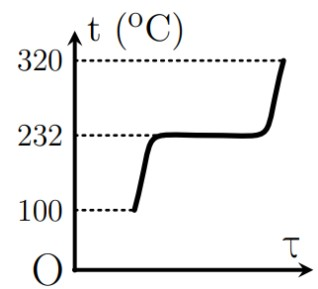
\includegraphics[width=0.2\linewidth]{../figs/D12-5-1}	
	\end{center}
	\choice
	{$\SI{210}{\celsius}$}
	{$\SI{100}{\celsius}$}
	{$\SI{320}{\celsius}$}
	{\True $\SI{232}{\celsius}$}
	\loigiai{}
\end{ex}
% ===================================================================
\begin{ex}
	Thực hiện công $\SI{170}{\joule}$ lên khối khí trong xilanh làm nội năng khối khí tăng thêm $\SI{170}{\joule}$. Chọn kết luận đúng
	\choice
	{Khối khí nhận nhiệt lượng $\SI{170}{\joule}$}
	{Khối khí tỏa nhiệt lượng $\SI{340}{\joule}$}
	{Khối khí nhận nhiệt lượng $\SI{340}{\joule}$}
	{\True Khối khí không trao đổi nhiệt lượng với môi trường}
	\loigiai{}
\end{ex}
% ===================================================================
\begin{ex}
	Một lượng khí lý tưởng ở nhiệt độ $\SI{100}{\celsius}$ và áp suất $\SI{E5}{\pascal}$ được nén đẳng nhiệt đến áp suất $\SI{1.5E5}{\pascal}$. Hỏi sau đó phải làm lạnh đẳng tích khí đó đến nhiệt độ nào để áp suất bằng lúc đầu?
	\choice
	{$\SI{24}{\celsius}$}
	{\True $\SI{-24}{\celsius}$}
	{$\SI{-12}{\celsius}$}
	{$\SI{36}{\celsius}$}
	\loigiai{
	\begin{center}
		\begin{tabular}{|M{5.5cm}|M{5.5cm}|M{5.5cm}|}
			\hline
			$p$ & $V$ & $T$\\
			\hline
			$\SI{E5}{\pascal}$ & $V_1$ & $100+273=\SI{373}{\kelvin}$\\
			\hline
			$\SI{1.5E5}{\pascal}$ & $V$ & $\SI{373}{\kelvin}$\\
			\hline
			$\SI{E5}{\pascal}$ & $V$ & $T_3$\\
			\hline
		\end{tabular}
	\end{center}
	$$\dfrac{p_3}{T_3}=\dfrac{p_2}{T_2}\Leftrightarrow\dfrac{10^5}{T_3}=\dfrac{1,5\cdot10^5}{373}\Rightarrow T_3\approx\SI{249}{\kelvin}\Rightarrow t_3\approx\SI{-24}{\celsius}.$$
	}
\end{ex}
% ===================================================================
\begin{ex}
	\immini{Hình vẽ là đồ thị biểu diễn sự thay đổi áp suất $p$ theo nhiệt độ tuyệt đối $T$ của một khối khí lí tưởng. Khối khí này bắt đầu biến đổi từ trạng thái A, sang trạng thái B, rồi chuyển sang trạng thái C với khối lượng riêng ở các trạng thái tương ứng là $\rho_{\mathrm{A}}$, $\rho_{\mathrm{B}}$, $\rho_{\mathrm{C}}$. So sánh đúng là}
	{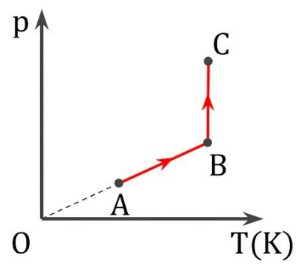
\includegraphics[width=0.45\linewidth]{../figs/D12-5-7}}
	\choice
	{$\rho_{\mathrm{A}}>\rho_{\mathrm{B}}>\rho_{\mathrm{C}}$}
	{\True $\rho_{\mathrm{A}}=\rho_{\mathrm{B}}<\rho_{\mathrm{C}}$}
	{{$\rho_{\mathrm{A}}<\rho_{\mathrm{B}}=\rho_{\mathrm{C}}$}}
	{{$\rho_{\mathrm{A}}=\rho_{\mathrm{B}}=\rho_{\mathrm{C}}$}}
	\loigiai{
	$\rho=\dfrac{m}{V}\Rightarrow V$ càng bé thì $\rho$ càng lớn.\\
	AB là quá trình đẳng tích $\Rightarrow V_{\mathrm{A}}=V_{\mathrm{B}}\Rightarrow \rho_{\mathrm{A}}=\rho_{\mathrm{B}}$\\
	BC là quá trình đẳng nhiệt $\Rightarrow pV=const$ mà $p_{\mathrm{B}}<p_{\mathrm{C}}\Rightarrow V_{\mathrm{B}}>V_{\mathrm{C}}\Rightarrow \rho_{\mathrm{B}}<\rho_{\mathrm{C}}$.
	}
\end{ex}
% ===================================================================
\begin{ex}
	\immini{Một bình chứa khí được chia làm 2 ngăn A và B bởi piston cách nhiệt. Ban đầu, piston bị chốt lại để thể tích khí ở ngăn A gấp 1,5 lần thể tích khí ở ngăn B. Lúc này, khí ở ngăn A có nhiệt độ $\SI{177}{\celsius}$ và áp suất $\SI{1.5}{atm}$,  khí ở ngăn B có nhiệt độ $\SI{27}{\celsius}$ và áp suất $\SI{1.2}{atm}$. }
	{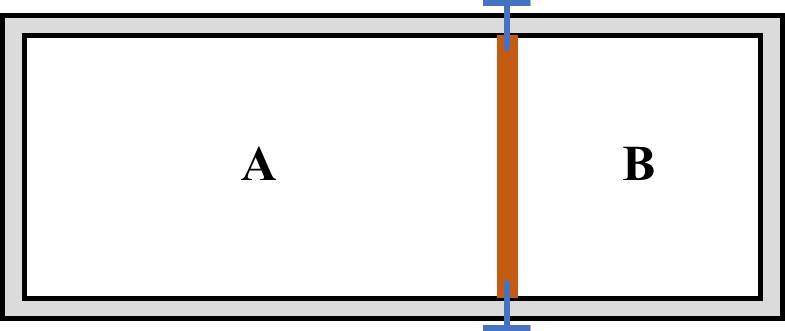
\includegraphics[width=0.5\linewidth]{{../figs/D12-5-8}}}
	Người ta tháo chốt để piston chuyển động tự do trong bình. Do thành bình dẫn nhiệt chậm nên khí A và B cuối cùng đạt đến nhiệt độ phòng là $\SI{27}{\celsius}$. Khi piston dừng lại, áp suất khí trong mỗi bình là
	\choice
	{$\SI{1.12}{atm}$}
	{$\SI{1.05}{atm}$}
	{\True $\SI{1.08}{atm}$}
	{$\SI{0.90}{atm}$}
	\loigiai{
	\begin{center}
		\begin{tabular}{|M{4cm}|M{4cm}|M{4cm}|M{4cm}|}
			\hline
			\thead{Trạng thái}& $p$ & $V$ & $T$\\
			\hline
			Phần A ban đầu & $\SI{1.5}{atm}$& $3V$ &$\SI{450}{\kelvin}$\\
			\hline
			Phần B ban đầu & $\SI{1.2}{atm}$ & $2V$ & $\SI{300}{\kelvin}$\\
			\hline
			Phần A lúc sau & $p'$ & $V'_{\mathrm{A}}$ & $\SI{300}{\kelvin}$\\
			\hline
			Phần B lúc sau & $p'$ & $V'_{\mathrm{B}}$& $\SI{300}{\kelvin}$\\
			\hline
		\end{tabular}
	\end{center}
	$$\dfrac{pV}{T}=const\Rightarrow \begin{cases}
		\frac{1,5\cdot3V}{450}=\frac{p'\cdot V'_{\mathrm{A}}}{300}\\
		\frac{1,2\cdot2V}{300}=\frac{p'\cdot V'_{\mathrm{B}}}{300}
	\end{cases}\Rightarrow\begin{cases}
	V'_{\mathrm{A}}=\frac{3V}{p'}\\
	V'_{\mathrm{B}}=\frac{2,4V}{p'}
	\end{cases}$$
	Mà:
	$$V'_{\mathrm{A}}+V'_{\mathrm{B}}=3V+2V\Leftrightarrow\dfrac{3}{p'}+\dfrac{2,4}{p'}=3+2\Rightarrow p'=\SI{1.08}{atm}.$$
	}
\end{ex}
\Closesolutionfile{ans}
\section{Câu trắc nghiệm đúng/sai} 
\textit{Thí sinh trả lời từ câu 1 đến câu 4. Trong mỗi ý \textbf{a)}, \textbf{b)}, \textbf{c)}, \textbf{d)} ở mỗi câu, thí sinh chọn đúng hoặc sai}
\setcounter{ex}{0}
\Opensolutionfile{ans}[ans/G12-5-TF]
% ===================================================================
\begin{ex}
Cho các phát biểu sau, phát biểu nào đúng? Phát biểu nào sai?	
	\choiceTF[t]
	{Nhiệt hoá hơi riêng của một chất tăng khi nhiệt độ tăng}
	{\True Nhiệt hoá hơi riêng của một chất lỏng là nhiệt lượng cần để làm cho $\SI{1}{\kilogram}$ chất lỏng đó hoá hơi hoàn toàn ở nhiệt độ xác định}
	{Nhiệt lượng cần cung cấp cho một lượng chất lỏng hoá hơi ở nhiệt độ không đổi, không phụ thuộc vào khối lượng và bản chất của chất lỏng}
	{\True Sự hóa hơi được ứng dụng trong các thiết bị làm lạnh (máy điều hoà nhiệt độ, dàn lạnh, dàn bay hơi,.), nồi hấp tiệt trùng trong y học, thiết bị xử lí rác thải ứng dụng công nghệ hoá hơi}
	\loigiai{}
\end{ex}
% ===================================================================
\begin{ex}
	Khi nung nóng một khối khí chứa trong một xilanh có pit-tông đóng kín làm cho nhiệt độ của khối khí tăng. Pit-tông này có thể dịch chuyển không ma sát trong xilanh.
	\begin{center}
		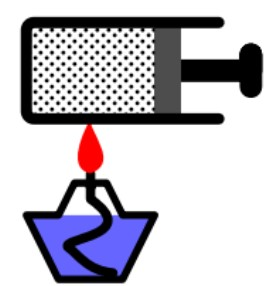
\includegraphics[width=0.15\linewidth]{../figs/D12-5-2}
	\end{center}
	\choiceTF[t]
	{\True Nhiệt độ của khối khí trong xilanh thay đổi do quá trình truyền nhiệt}
	{\True Khi cho pit-tông chuyển động tự do để khối khí dãn nở với áp suất không đổi, lúc này khối khí đã sinh công}
	{\True Khi giữ pit-tông để thể tích khí không đổi thì toàn bộ nhiệt lượng khối khí nhận được dùng để tăng nội năng của khí (khối khí không tỏa nhiệt)}
	{Khi nhận nhiệt, động năng của các phân tử là không đổi}
	\loigiai{}
\end{ex}
% ===================================================================
\begin{ex}
	Giả sử một học sinh tạo ra một nhiệt kế sử dụng một thang nhiệt độ mới cho riêng mình, gọi là thang nhiệt độ Z, có đơn vị là $\si{\degree Z}$. Trong đó, nhiệt độ của nước đá đang tan ở $\SI{1}{atm}$ là $\xsi{x}{\degree Z}$ và nhiệt độ nước sôi ở $\SI{1}{atm}$ là $\xsi{y}{\degree Z}$. Từ vạch $\xsi{x}{\degree Z}$ đến vạch $\xsi{y}{\degree Z}$ được chia thành 180 khoảng, mỗi khoảng ứng với $\SI{1}{\degree Z}$.
	\choiceTF[t]
	{Một độ chia trên thang nhiệt độ Z bằng 1,8 lần độ chia trên thang nhiệt độ Celsius}
	{\True Mối liên hệ giữa $x$ và $y$ là: $y=x+180$}
	{Độ biến thiên nhiệt độ $\SI{18}{\celsius}$ trong thang nhiệt độ Celsius bằng với độ biến thiên nhiệt độ $\SI{10}{\degree Z}$ trong thang nhiệt độ Z}
	{\True Nếu nhiệt độ cơ thể người là $\SI{37}{\celsius}$ tương ứng với $\SI{86.6}{\degree Z}$ thì giá trị của $x$ là 20 }
	\loigiai{
	\begin{itemchoice}
		\itemch Sai. Gọi $a$ là mỗi độ chia trong thang Z và $b$ là mỗi độ chia trong thang Celsius thì $180a=100b\Rightarrow a=\dfrac{b}{1,8}$.
		\itemch Đúng.
		\itemch Sai. $18b=\Delta z. a\Rightarrow \Delta z=1,8\cdot18=32,4$.
		\itemch Đúng. $\dfrac{86,6-x}{180}=\dfrac{37-0}{100}\Rightarrow x=20$.
	\end{itemchoice}
	}
\end{ex}
% ===================================================================
\begin{ex}
Khi tiến hành nung nóng một chất rắn kết tinh bằng một bếp có công suất không đổi. Bỏ qua sự mất mát nhiệt lượng ra môi trường. Kể từ lúc bắt đầu đun người ta ghi nhận được đồ thị sự phụ thuộc của nhiệt độ của khối chất và thời gian đun như hình bên.	
\begin{center}
	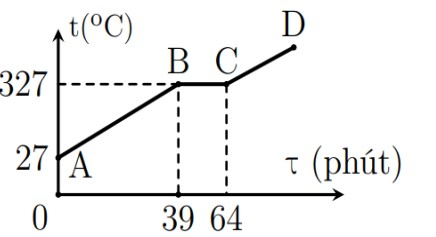
\includegraphics[width=0.3\linewidth]{../figs/D12-5-3}
\end{center}
	\choiceTF[t]
	{\True Nhiệt độ nóng chảy của chất rắn trên là $\SI{327}{\celsius}$}
	{\True Kể từ lúc bắt đầu đun, nhiệt lượng cần để chất rắn tăng lên đến nhiệt độ nóng chảy gấp 1,56 lần nhiệt lượng cần cung cấp trong suốt giai đoạn nóng chảy}
	{Đoạn AB trên đồ thị thể hiện quá trình chất rắn đang nóng chảy}
	{Tại phút thứ 39 chất rắn đã nóng chảy hoàn toàn}
	\loigiai{}
\end{ex}

\Closesolutionfile{ans}
\section{Câu trắc nghiệm trả lời ngắn} \textit{Thí sinh trả lời từ câu 1 đến câu 6}
\setcounter{ex}{0}
\Opensolutionfile{ans}[ans/G12-5-TL]
% ===============================================================
\begin{ex}
	Biết nhiệt dung riêng của nước là $\SI{4190}{\joule/\kilogram\cdot\kelvin}$ và nhiệt hóa hơi riêng của nước là $\SI{2.26E6}{\joule/\kilogram}$. Cần cung cấp một nhiệt lượng bằng bao nhiêu $\si{\mega\joule}$ để làm cho $\SI{200}{\gram}$ nước có nhiệt độ $\SI{10}{\celsius}$ sôi ở $\SI{100}{\celsius}$ và $\SI{10}{\percent}$ khối lượng của nó đã hóa hơi khi sôi? \textit{(Kết quả lấy đến 2 chữ số sau dấu phẩy thập phân)}.
	\shortans{$0,12$ }
	\loigiai{
	$Q=mc\Delta t+\SI{10}{\percent}mL\approx\SI{0.12}{\mega\joule}.$
	}
\end{ex}
% ===============================================================
\begin{ex}
Truyền cho khí trong xi lanh một nhiệt lượng $\SI{200}{\joule}$. Khí nở ra và thực hiện công $\SI{140}{\joule}$ đẩy pittông lên. Độ biến thiên nội năng của khí là bao nhiêu $\si{\joule}$?
	\shortans{$60$ }
	\loigiai{
		Độ biến thiên nội năng của khí:
		$$\Delta U=Q+A=Q-A'=\SI{60}{\joule}.$$
	}
\end{ex}
% ===============================================================
\begin{ex}
	Một số nước trên thế giới sử dụng thang đo nhiệt độ Fahrenheit. Trong thang nhiệt này (ở áp suất tiêu chuẩn) nhiệt độ của nước đá đan tan là $\SI{32}{\degree F}$, của nước đang sôi là $\SI{212}{\degree F}$. Công thức chuyển đổi giữa thang đo Fahrenheit và thang đo Celsius là: $t\left(\si{\degree F}\right)=32+1,8 \cdot t\left(\si{\celsius}\right)$. Nhiệt độ bằng bao nhiêu $\si{\celsius}$ thì giá trị nhiệt độ trên hai thang đo là bằng nhau?
	\shortans{$-40$ }
	\loigiai{
		$$t=32+1,8 \cdot t\Rightarrow t=\SI{-40}{\celsius}.$$}
	\end{ex}
	% ===============================================================
	\begin{ex}
	\immini{
	Hình bên là đồ thị biểu diễn sự phụ thuộc của nhiệt độ vào thời gian đun một ấm nước ở áp suất tiêu chuẩn. Nếu nhiệt lượng mà bếp tỏa ra không thay đổi trong suốt thời gian đun thì sau bao nhiêu giây kể từ lúc bắt đầu đun nước sẽ sôi?
	}
	{
	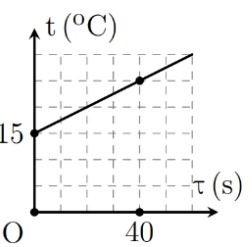
\includegraphics[width=0.4\linewidth]{../figs/D12-5-4}
	}
		\shortans{$340$ }
		\loigiai{
			Thời gian đun $\left(\dfrac{100-15}{10}\right)\cdot40=\SI{340}{\second}.$
		}
	\end{ex}
	% ===============================================================
	\begin{ex}
		\immini{
		Bằng các nghiên cứu, người ta phát hiện ra rằng các nguyên tử của nguyên tố X sắp xếp tuần hoàn tạo thành mạng tinh thể gồm các ô hình lập phương giống hệt nhau xếp chồng lên nhau (Hình a). Ở mỗi ô lập phương nhỏ nhất (gọi là ô mạng cơ sở) có một nguyên tử nằm tại tâm và ở mỗi đỉnh của nó đều có một nguyên tử (Hình b). 
		}{
		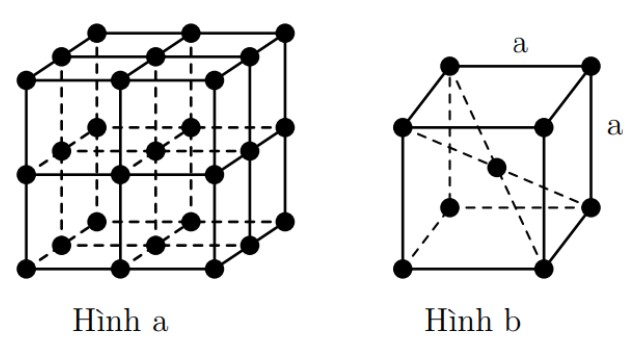
\includegraphics[width=0.6\linewidth]{../figs/D12-5-5}
		}
		Biết rằng chiều dài cạnh của mỗi ô lập phương cơ sở là $a=\SI{2.87E-10}{\meter}$. Biết khối lượng mỗi nguyên tử X là $\SI{9.3E-26}{\kilogram}$. Khối lượng riêng của nguyên tố X là bao nhiêu $\si{\kilogram/\meter^3}$? \textit{(Kết quả chỉ lấy phần nguyên)}.
		\shortans{$7868$}
		\loigiai{
		Một ô mạng có thể tích là $a^3$ gồm:
		\begin{itemize}
			\item 8 nguyên tử ở đỉnh, mỗi nguyên tử ở đỉnh chỉ đóng góp 1/8 cho ô mạng.
			\item 1 nguyên tử ở tâm của ô mạng.
		\end{itemize}	
		$\Rightarrow$ tổng đóng góp cho 1 ô mạng là $8\cdot \dfrac{1}{8}+1=2$ nguyên tử.\\
		$D=\dfrac{2m_X}{a^3}\approx\SI{7868}{\kilogram/\meter^3}$.
		}
	\end{ex}
	% ===============================================================
	\begin{ex}
		\immini{
		Một xilanh có pittong gắn với một lò xo có độ cứng $\SI{2E3}{\newton/\meter}$. Cho diện tích của pittong là $\SI{0.01}{\meter^2}$ và khối lượng của nó không đáng kể. Ban đầu, lò xo ở trạng thái không biến dạng, lượng khí trong xilanh có thể tích $\SI{5}{\liter}$ ở áp suất khí quyển $p_0=\SI{1}{atm}$ và nhiệt độ $\SI{20}{\celsius}$. Khi tăng nhiệt độ lên đến $\SI{250}{\celsius}$ thì pittong dịch chuyển được một đoạn bao nhiêu $\si{\meter}$ \textit{(làm tròn đến 2 chữ số sau dấy phẩy thập phân)}?
		}{
		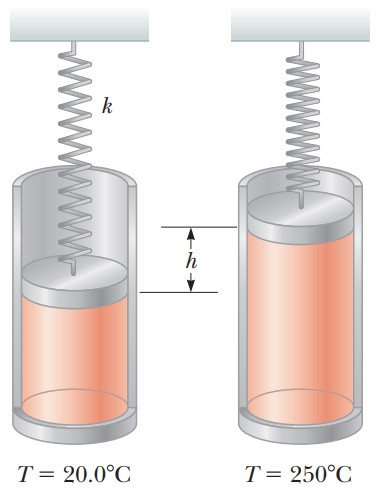
\includegraphics[width=0.4\linewidth]{../figs/D12-5-6}
		}
		\shortans{$0,17$ }
		\loigiai{
			\begin{center}
				\begin{tabular}{|M{5.5cm}|M{5.5cm}|M{5.5cm}|}
				\hline
				$p$ & $V$&$T$\\
				\hline
				$\SI{101325}{\pascal}$ & $\SI{5E-3}{\meter^3}$ & $\SI{293}{\kelvin}$\\
				\hline
				$p_0+\dfrac{kh}{S}=101325+\dfrac{2\cdot10^3h}{0,01}\ \si{\pascal}$ & $\SI{5E-3}{}+0,01h\ \si{\meter^3}$&$\SI{523}{\kelvin}$\\
				\hline
				\end{tabular}
			\end{center}
			$$\dfrac{pV}{T}=const\Rightarrow \dfrac{101325\cdot5\cdot10^{-3}}{293}=\dfrac{\left(101325+\dfrac{2\cdot10^3h}{0,01}\right)\cdot\left(5\cdot10^{-3}+0,01h\right)}{523}\Rightarrow h\approx\SI{0.17}{\meter}.$$
		}
	\end{ex}
\Closesolutionfile{ans}
\begin{center}
	\textbf{-- HẾT --}
\end{center}
